\documentclass[Ex4_Zusammenfassung.tex]{subfiles}

\begin{document}

\chapter{Werkzeuge der Kern- und Teilchenphysik} 
\textbf{von \hein \& \mitsch}

\section{Zerfallsgesetz}
Es gibt 3 verschiedene Arten des radioaktiven Zerfalls.  (A: Nukleonenanzahl , Z: Kernladungszahl)
\begin{itemize}
\item  $ \alpha $  - Zerfall:  $ ^{A}_{Z}X \rightarrow ^{A-4}_{Z-2}Y \ + \ ^{4}_{2}He^{++} $    \\ $ \alpha $ -Strahlung wird mittlels Heliumkernen vermittelt (positiv geladen). 
\item $ \beta $ - Zerfall: 
	\begin{enumerate} 
	\item $ \beta^{-} $ - Zerfall: $ ^{A}_{Z} X\rightarrow ^{A}_{Z+1} Y\ + \ e^{-} \ +\overline{\nu_{e}} $  \\ Beim  $ \beta^{-} $ -Zerfall wird im Kern ein Neutron in ein Proton umgewandelt. Dabei werden ein Elektron und ein Elektron-Antineutrino emittiert.
	\item $ \beta^{+} $ - Zerfall: $ ^{A}_{Z}X \rightarrow ^{A}_{Z-1}Y \ + \ e^{+} \ +\nu_{e} $ \\ Beim $ \beta^{+} $ -Zerfall wird im Kern ein Proton in ein Neutron umgewandelt. Dabei werden ein Positron und ein Elektron-Neutrino emittiert.
	\end{enumerate}
\item $ \gamma $ -Zerfall :  $ ^{A}_{Z}X^{*} \rightarrow ^{A}_{Z}X + \gamma $ \newline Falls nach einem $ \alpha $ - Zerfall oder $ \beta $ - Zerfall ein Atomkern in einem angeregten Zustand vorliegt, ist $ \gamma $ - Zerfall möglich. Beim Übergang in einen energetisch günstigeren Zustand wird hochfrequente elektromagnetische Strahlung emittiert. Meist folgt der  $ \gamma $ -Zerfall unmittelbar auf einen $ \alpha $ - oder $ \beta $ - Zerfall. \\ 
\newline 
Für die Zerfallsrate(Aktivität) $ A = \derive{}{t} N(t)$  gilt die folgende Differentialgleichung: 
\begin{equation}
\derive{}{t} N(t) = - \lambda N(t) 
\end{equation}
$ \lambda $ : Zerfallskonstante beschreibt Wahrscheinlichkeit für eine bestimmte radioaktive Zerfallsart. Sie ist unabhängig von Ort und Zeit, aber charakteristisch für den Kern. \newline
Die Lösung dieser Gleichung gibt die Anzahl N der Atome zum Zeitpunkt t an: 
\begin{equation}
N(t) = N_{0} e^{-\lambda \cdot t}
\end{equation}  
Wobei man in diesem Zusammenhang noch folgende nützliche Größen definiert: 
\begin{itemize}
\item Mittlere Lebensdauer: $ \tau = \nicefrac{1}{\lambda} $ \newline 
Nach dieser Zeit sind nur noch $\nicefrac{1}{e} $ ($ \approx 37 \% $) der ursprünlichen Atome vorhanden.
\item Halbwertszeit : $ T_{\nicefrac{1}{2}} = \frac{ln(2)}{\lambda} $
Nach dieser Zeit sind nurnoch 50 \% der ursprünlichen Atome vorhanden.
\end{itemize}
\end{itemize}
Der radioaktive Zerfall ist ein stat. Prozess. Die Wahrscheinlichkeit einen zerfallenden Kern anzutreffen ist bei t=0 am größten, danach fällt sie exponentiell ab. 
Diese Wahrscheinlichkeit ist prinzipiell eine Binomial-Verteilung. Für eine hohe Anzahl an Versuchen und eine kleine Wahrscheinlichkeit konvergiert die Binomialverteilung gegen eine Poisson-Verteilung. Diese Näherung lässt sich auf den radioaktiven Zerfall anwenden, da man in der Regel viele Atome (N $\approx 10^{23} $) betrachtet, also eine hohe Anzahl Versuche durchführt, und die Zerfallswahrscheinlichkeit in der Regel klein ist: 
\begin{equation}
p(t) = 1 - e^{-\lambda \cdot t} 
\end{equation}
Somit lässt sich der Zerfall also durch eine Poisson-Verteilung beschreiben mit dem Mittelwert $ \mu = N\cdot p $ und der Standardabweichung  $ \sigma = \sqrt{\mu} $ wobei der Zerfall k-mal eintreten soll. 
\begin{equation}
P(k) = \frac{\mu^k \cdot e^{-\mu} } {k!} 
\end{equation}

\section{Fermis Goldene Regel}
Wir wollen eine Vorraussage für die Übergangsrate $ \lambda $ (Übergangswahrscheinlichkeit pro Zeit), mit der ein Anfangszustand unter dem Einfluss einer Störung in einen anderen Zustand übergeht, treffen. Wir nehmen dabei an, dass es sich um ein an sich zeitlich konstantes System handelt, welches durch den Hamilton-Operator $ H_0 $ beschrieben wird, und durch einen Störoperator V, welcher vergleichsweise klein gegenüber  $ H_0 $ ist, gestört wird. Der gesamte Hamiltonoperator lautet also $ H = H_0 + V $ \newline
Wir formulieren Fermis Goldene Regel: 
\begin{equation}
\lambda_{A\rightarrow E} = \frac{2\pi}{\hslash} \cdot |\braket{\psi_{E} | V |\psi_{A}}|^2 \cdot \rho_{E} = \derive{P}{t}
\end{equation}
Die Übergansrate hängt also davon ab wie stark die Störung V den Anfangszustand $\ket{\psi_A}\ \lp \equiv \ket{i} \text{ für initial } \rp $ und den Endzustand $ \ket{\psi_E }\ \lp \equiv \ket{f} \text{ für final } \rp $ koppelt. Außerdem skaliert die Übergangsrate mit der Anzahl der möglichen Übergänge welche durch die Endzustandsdichte $ \rho_{E} $ beschrieben wird. 

\subsubsection*{Was ist $\rho(E)$ eigentlich?}
Wir bezeichnen den Phasenraum unseres Systems als den Raum, der durch die Ortskoordinaten \textbf{x} und die dazugehörigen Impulse \textbf{p} aufgespannt wird. In diesem Raum können wir einem Punkt ein Volumen von $ h^3 = (2\pi \hslash)^3 $ zuordnen (Unschärferelation). \newline 

\textbf{1 Dimension}:

Zunächst betrachten wir einen jeweils eindimensionalen Orts-und Impulsraum mit Zuständen $ (x,p) \in  [x,x+L] \times [p_{x},p_{x}+p] $ In diesem Fall kann die Gesamtfläche Lp mit $ N = \frac{Lp}{2\pi \hslash} $ Zuständen gefüllt werden. Für die Zustandsdichte gilt dann: 
\begin{equation}
	 \rho(E) = \derive{N}{E} = 2 \derive{N}{p} \derive{p}{E} = \frac{L}{2\pi \hslash} \frac{2m}{p} =  \frac{L}{2\pi \hslash} \sqrt{\frac{2m}{E}} 
 \end{equation}
 Wobei wir im letzten Schritt auf Kugelkoordinaten transformieren. 
 Der Faktor 2 kommt daher, dass die Zustände (x,p) und (x,-p) bezüglich der Energie entartet sind, denn $ E = E_{kin} = \frac{p^2}{2m} $ \newline
 
 \textbf{3 Dimensionen}:
 
 Die Anzahl der Gesamtzustände N ist nun
 \begin{equation}
	 N = \frac{1}{(2 \pi \hslash)^3} \int \md\textbf{x}^3 \md\textbf{p}^3 = \frac{V}{(2 \pi \hslash)^3} \int \md\textbf{p}^3 = \frac{V}{(2 \pi \hslash)^3} \int p^2 \md p   \md\Omega 
 \end{equation}
 Aus der relativistischen Energie-Impuls-Beziehung $ E^2 = (pc)^2 +  (m_pc^2)^2 $ folgern wir $ \frac{d}{dE} = \frac{E}{pc^2} \frac{d}{dp} $ und erhalten damit für die Zustandsdichte für \textbf{1 Teilchen}
\begin{equation}
	\rho(E) = \derive{N}{E} = \frac{V}{(2 \pi \hslash)^3}  \frac{E}{pc^2} \derive{}{p}  \int p^2 \md p \  \md\Omega =  \frac{V}{(2 \pi \hslash)^3} \frac{pE}{c^2} \int \md \Omega = \frac{VpE}{2 \pi^2 c^2 \hslash^3}
\end{equation}

Für \textbf{2 Teilchen} addieren sich die Impulse im Mittel zu 0, weshalb die Zustandsdichte konstant ist. Jedoch addieren sich die Energien zu $ E = E_1 + E_2 $
\begin{equation}
	\md E = \md E_1 + \md E_2 = \frac{p_1c^2}{E_1} \md p_1 + \frac{p_2c^2}{E_2} \md p_2
\end{equation}
Da $ p_1^2 = p_2^2 $ folgt $  p_1 \md p_{1} = p_2 \md p_{2} $ 
\begin{align*}
	\rightarrow \md E &= \frac{E_1 + E_2}{E_1E_2} c^2 p_1 \md p_1  \\
	\rightarrow  \rho_2 &=   \frac{V}{(2 \pi \hslash)^3} \frac{E_1E_2}{E_1+E_2} p_{1} \int \md\Omega_{1}
\end{align*}
Wir können dies auf n Teilchen erweitern
\begin{equation}
	\rho_{n} = \frac{V^{n-1}}{(2 \pi \hslash)^{3(n-1)}} \derive{}{E} \prod_{i=1}^{n-1} \int \md^3 \textbf{p}_{i} 
\end{equation}

\section{Wirkungsquerschnitt}
Die bisherigen Überlegungen dienten allesamt dazu die Reaktionsrate einer Zustandsänderung zu quantifizieren. Wir lernen nun eine letzte Größe kennen, die ebenfalls diesen Zweck erfüllt.
Der Wirkungsquerschnitt $ \sigma $ gibt die Stärke einer Reaktion an. Um dies zu begreifen betrachten wir einen konstanten Fluss  $\Phi $ von Teilchen, die allesamt der Sorte P (projectile) zugehören und auf ein Target der Dicke x aus Teilchen der Sorte T (target) geschossen werden.  

\begin{figure}[h]
	\centering
	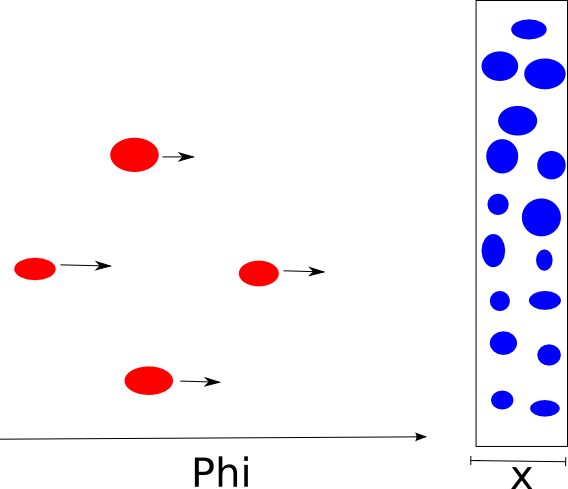
\includegraphics[height= 4cm, width=4cm]{fluss.png}
	\caption{Teilchenfluss auf Target}
\end{figure}
Die Reaktionsrate pro Targetteilchen ist 
\begin{equation}
	W = \Phi \cdot \sigma 
\end{equation}
Die Reaktionsrate im gesamten Target ist
\begin{equation}
	W \cdot N = \Phi \cdot n_{T} \cdot x \cdot \sigma 
\end{equation}
mit N Targetteilchen und der Volumenteilchendichte $ n_T $. Der Wirkungsquerschnitt $\sigma$ ist also die flussbereinigte Reaktionsrate. Er hat die Dimension [Fläche] und eine hierfür häufig verwendete Einheit heißt Barn $\SI{1}{b} = \SI{1E-24}{cm^2} = \SI{1E-28}{m^2}$.\\

Im Allgemeinen hängt der Wirkungsquerschnitt  $ \sigma $ von der Art der Reaktion ab: 
\begin{itemize}
\item Absorbtion $ \sigma_{A} $
\item elastische Streuung $ \sigma_{E} $
\item inelastische Streuung $ \sigma_{I} $
\end{itemize}
Der Gesamtwirkungsquerschnitt ergibt sich via Addition $ \sigma_{Ges} = \sigma_{A} + \sigma_{E} + \sigma_{I}  $ \newline
Für Teilchen die sich innerhalb eines Mediums ausbreiten definiert man die \textbf{mittlere freie Weglänge} $\lambda$
\begin{equation}
	\lambda = \frac{1}{n_T \sigma}
\end{equation} 
Diese gibt die durchschnittliche Strecke an, die ein Teilchen im Target ohne Wechselwirkung zurücklegen kann. \\

Das Volumen in dem 1 Targetteilchen ist also $ V = \lambda \cdot \sigma = \nicefrac{1}{n_T} $  \newline
Anhand der mittleren freien Weglänge lassen sich folgende Größen berechnen: 
\begin{itemize}
	\item Anzahl der Strahlteilchen im Targetmaterial : $ N(x) = N_{0} \cdot e^{-\nicefrac{x}{\lambda}} $
	\item Kollisionsrate: $ c(x) = - \derive{N(x)}{x} = \frac{N_{0}}{\lambda} \cdot e^{-\nicefrac{x}{\lambda}} = c_0 \cdot e^{-\nicefrac{x}{\lambda}} $
	\item Wahrscheinlichkeit für Reaktion eines einfallenden Teilchens: $  p(x) = 1- e^{-\nicefrac{x}{\lambda}} $
\end{itemize}

Aus Dimensionsbetrachtungen lässt sich darauf schliessen, dass der Wirkungsquerschnitt die Dimension einer Fläche hat. Wir werden dies nun veranschaulichen: 
\begin{figure}[h]
	\centering
	\begin{tikzpicture}
		\draw[thick] (0cm,0cm) circle(3cm);
		\draw[fill=blue] (0cm,-1.5cm) circle(0.5cm);
		\draw [pattern=north west lines] (0cm,1cm) circle(1cm);
		\draw[fill=blue] (-1.5 cm,-1.5cm) circle(0.5cm);
		\draw[fill=blue] (1.5cm,-1.0cm) circle(0.5cm);
		\draw[fill=red] (0cm,2.0) circle(0.25cm);
		\draw[fill=blue] (0cm,1cm) circle(0.75cm);
		
		\draw [->] (-4.3,1.3) -- (-1,1);
		\draw [->] (-4.3,-1.3) -- (-0.4,0.7);
		\draw [->] (4.5,2.0) -- (0.3,2.0);
		\node at (4.5,0) {Targetfläche A};
		\node at (-4.5,-1.5) {Targetkern};
		\node at (-4.5,1.5) {Wirkungsquerschnitt};
		\node at (4.5,2.2) {Auftreffendes Teilchen};
	\end{tikzpicture}
	\caption{Wirkungsquerschnitt eines Teilchens (rot) das auf ein Targetteilchen (blau) trifft, mit Wirkungsquerschnitt (gewellte Fläche)}
\end{figure} \newline
Im Allgemeinen ist bei Teilchenkollisionen der Wirkungsquerschnitt, die kleinste Fläche, die beide Teilchen komplett einschließt: 
\begin{equation}
\sigma = \pi (r_{K} + r_{P})^2 
\end{equation}
wobei $ r_K $ der Kernradius und $ r_P $ der Projektilradius sind. 

Hieraus ergibt sich die Wahrscheinlichkeit, dass n Projektile mit dem Target wechselwirken, als das Verhältnis der effektiven Flächen:
\begin{equation}
	P = \frac{n_T \sigma}{A} = \lp \frac{n}{A} \rp_T \sigma
\end{equation}
\end{document}